\renewcommand{\baselinestretch}{2} \small\normalsize
\chapter{Propagation Statistics}
This chapter describes the propagation factor statistics after numerically propagating over independent random sea surface realizations generated following \cite{frazier_ocean} in a Monte Carlo fashion. First we will discuss the sampling constraints needed to capture the statistics appropriately and then look at the Monte Carlo run setup and provide some example data before finally fitting the PDFs.

\section{Sampling Constraints}
The initial set of runs was performed at Ka-Band (35 GHz) and the mean and standard deviation for a 100 run Monte Carlo set are shown in Figure \ref{stat_fig:1}. This data set took over 48 hours to complete running on a laptop and the results were washed out at near range (Figure \ref{stat_fig:1} is clipped at 10 km in near range).

\begin{figure}[H]
  \begin{center}
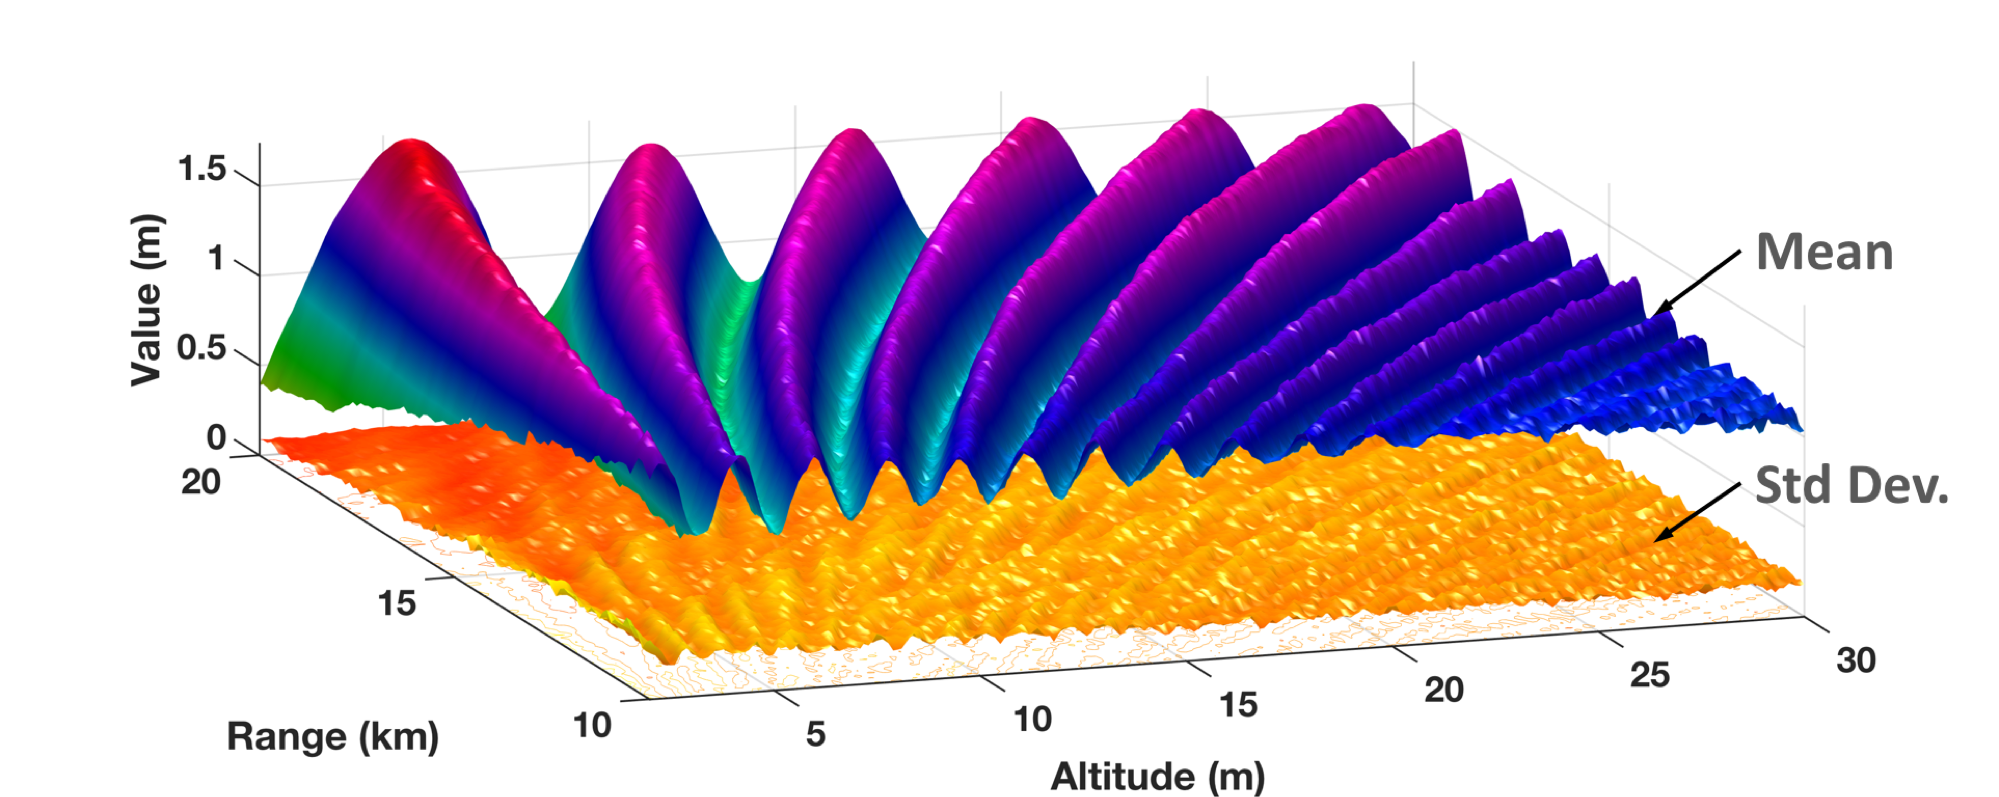
\includegraphics[width=5in]{../media/statistics/ka_band_stats.png}
  \end{center}
  \renewcommand{\baselinestretch}{1} \small\normalsize
  \begin{quote}
    \caption[Ensemble Statistics at Ka-Band with Standard Atmosphere]{Ensemble Statistics at Ka-Band with Standard Atmosphere\label{stat_fig:1}}
  \end{quote}
\end{figure}
\renewcommand{\baselinestretch}{2} \small\normalsize

Figure \ref{stat_fig:2} shows the mean and standard deviation for a 100 run Monte Carlo set at X-band (10 GHz). In this case, the near range results are much cleaner and the data set took less than 6 hours to complete.
\begin{figure}[H]
  \begin{center}
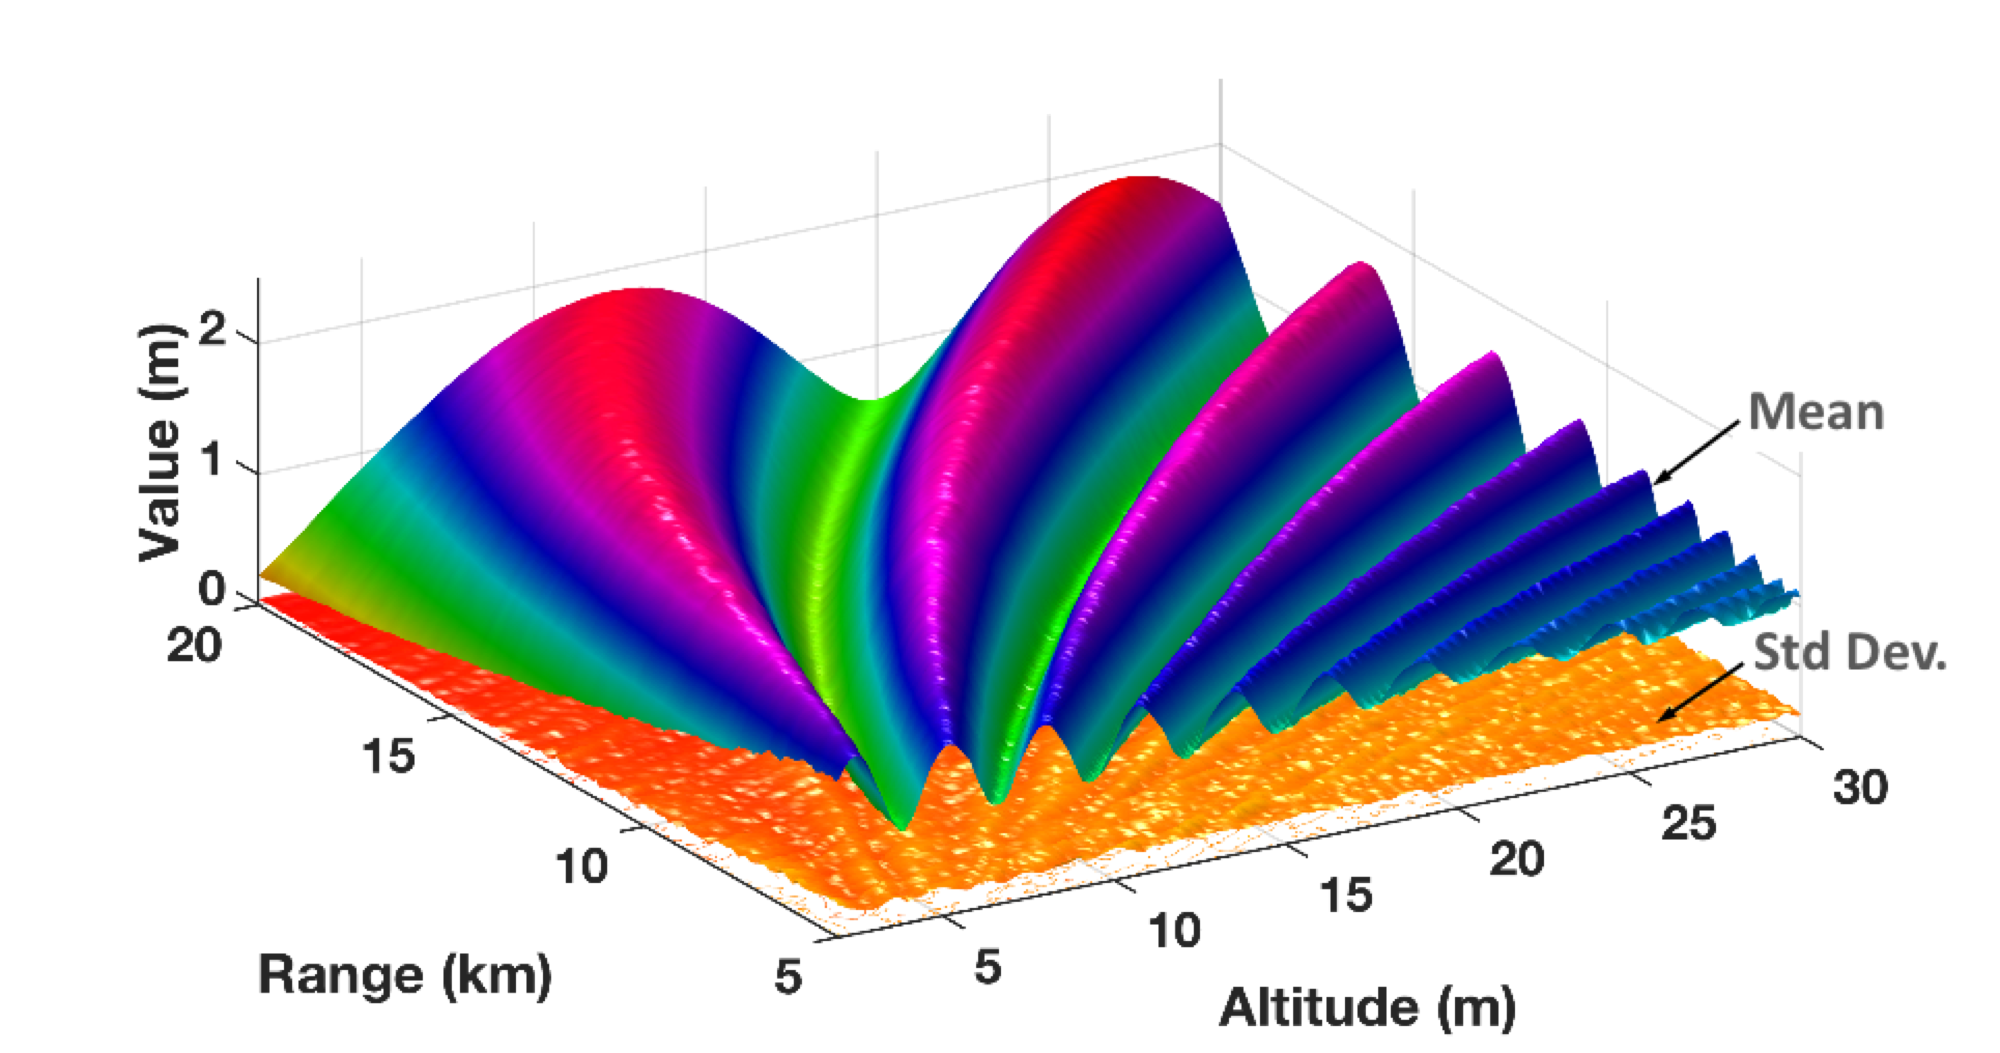
\includegraphics[width=5in]{../media/statistics/x_band_stats.png}
  \end{center}
  \renewcommand{\baselinestretch}{1} \small\normalsize
  \begin{quote}
    \caption[Ensemble Statistics at X-Band with Standard Atmosphere]{Ensemble Statistics at X-Band with Standard Atmosphere\label{stat_fig:2}}
  \end{quote}
\end{figure}
\renewcommand{\baselinestretch}{2} \small\normalsize

These results indicate that spatial sampling constraints from numerical propagation are important for obtaining accurate statistics. This does not mean the numerical propagation method is inaccurate, but that the solution is locally oscillatory so we need finer sampling to correctly capture variations.

To investigate the sampling constraints, we can look at the phase difference between the two primary paths from the propagation factor for the 2 ray model, $F_p = e^{jkL_1} + \Gamma_1e^{jkL_{so}}$. 

\begin{equation}
\begin{gathered}
\Delta\varphi = k\left[ L_1 - L_{so}\right] \\
\Delta\varphi = -\frac{4\pi h_1h_2}{\lambda L}
\label{stat_eq:1}
\end{gathered}
\end{equation}
\renewcommand{\baselinestretch}{2} \small\normalsize
The derivative of the phase difference with respect to range is then
\begin{equation}
\frac{d\Delta\varphi}{dL}=\frac{4\pi h_1h_2}{\lambda L^2}
\label{stat_eq:2}
\end{equation}
\renewcommand{\baselinestretch}{2} \small\normalsize

\noindent This equation can be converted from rad/m to rad/sample by multiplying by the spatial sampling distance in range, $\Delta r$. We can insist that this phase shift per sample be smaller than some pre-determined value to provide adequate sampling. It is often convenient to specify a limit in terms of wavelengths and we can enforce the condition that there must be at least $n$ samples per wavelength of phase difference by letting

\begin{equation}
\frac{4\pi h_1h_2\Delta r}{\lambda L^2} \leq \frac{2\pi \lambda}{n}
\label{stat_eq:3}
\end{equation}

This yields a constraint for the maximum allowable spatial sampling step to ensure $n$ samples per wavelength.
\begin{equation}
\boxed{\Delta r \leq \frac{\lambda^2 L^2}{2nh_1h_2}}
\label{stat_eq:4}
\end{equation}

This equation matches the observation with $n\approx 10$ for the mean values and $n\approx 20$ for the standard deviations. The sampling constraint is shown in Figure \ref{stat_fig:3} for both the 10 and 35 GHz cases, with $n = 20$ and $\Delta r = 0.5$.

\begin{figure}[H]
  \begin{center}
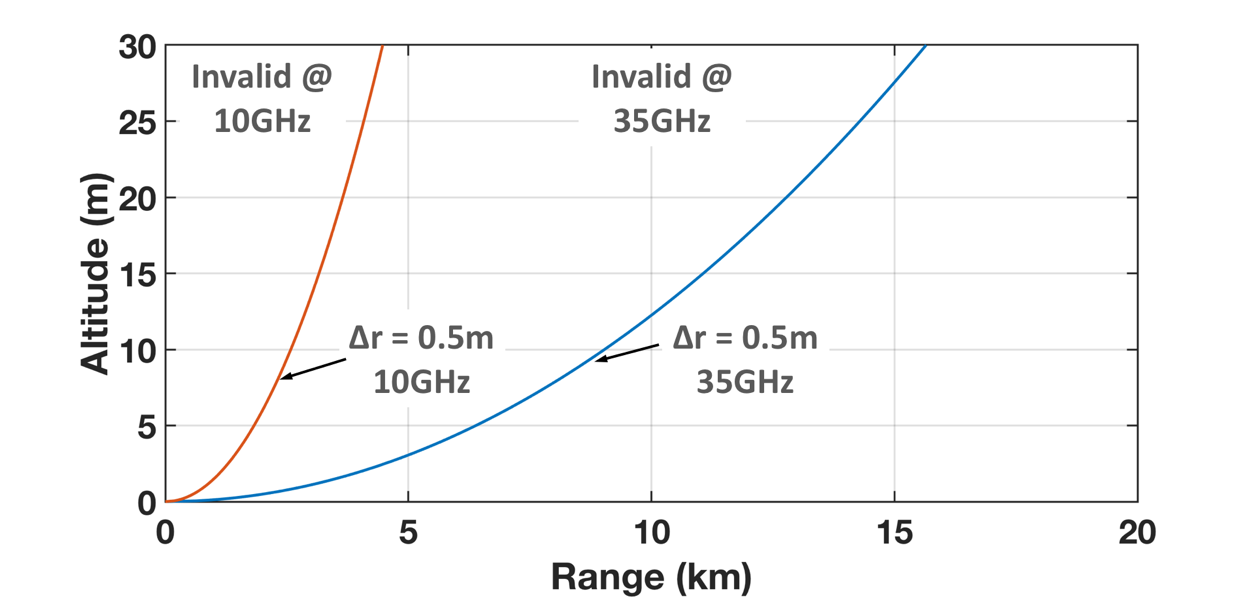
\includegraphics[width=5in]{../media/statistics/sampling_constraint.png}
  \end{center}
  \renewcommand{\baselinestretch}{1} \small\normalsize
  \begin{quote}
    \caption[Sampling Constraints for Statistical Analysis]{Sampling Constraints for Statistical Analysis\label{stat_fig:3}}
  \end{quote}
\end{figure}
\renewcommand{\baselinestretch}{2} \small\normalsize

\section{Monte Carlo Methodology}
The data set of propagation factors were generated by creating a random sea surface for a given wind speed and direction, and then numerically propagating using APL's Tropospheric Electromagnetic Parabolic Equation Routine (TEMPER), which is a Parabolic Wave Equation (PWE) solver. This sequence was repeated for 500 iterations with a different set of random variables for each sea surface.

\subsection{Input Parameters}
Table \ref{stat_tab:0} shows the common inputs that were used in all of the Monte Carlo runs.
\begin{table}[H]
  \begin{center}
      \renewcommand{\baselinestretch}{1} \small\normalsize
  \begin{quote}
    \caption[Common Monte Carlo Input Settings]{Common Monte Carlo Input Settings\label{stat_tab:1}}
  \end{quote}
  \begin{tabular} {|c | c |}
    \hline
  \bf{Parameter} & \bf{Value} \\ \hline
  Frequency & 10 GHz \\ \hline
  Antenna Pattern & Sinc \\ \hline
  Antenna Beamwidth & $8^{\circ}$  \\ \hline
  Polarization & Vertical \\ \hline
  Transmitter Height & 30 m \\ \hline
  Maximum Range & 20 km \\ \hline
  Range Step & 0.5 m  \\ \hline
  Maximum Altitude & 30 m \\ \hline
  Earth Model & Spherical \\ \hline
  Inverse Age Parameter & 0.84 (fully developed) \\ \hline
  Initial Seed & 561894\\ \hline
  Number of Runs & 500\\ \hline
\end{tabular}
\end{center}
\end{table}
\renewcommand{\baselinestretch}{2} \small\normalsize

The parameterizations resulted in 26 total data sets to capture the effect of wind speed (from 2 m/s to 15 m/s at $0^{\circ}$ wind direction), wind direction ($90^{\circ}$ to $0^{\circ}$ at 10 m/s wind speed), and refractive index profile (standard atmosphere and a 20 m duct). Table \ref{stat_tab:1} shows the primary run matrix with the various parameterizations. 
\begin{table}[H]
  \begin{center}
      \renewcommand{\baselinestretch}{1} \small\normalsize
  \begin{quote}
    \caption[Monte Carlo Propagation Run Matrix]{Monte Carlo Propagation Run Matrix\label{stat_tab:0}}
  \end{quote}
  \begin{tabular} {|c | c | c| c |}
    \hline
  \bf{Dataset ID} & \bf{Wind Speed} & \bf{Wind Direction} & \bf{Refractivity}  \\ \hline
  1 & 10 m/s & $0^{\circ}$ & Standard Atmosphere \\ \hline
  2 & 10 m/s & $18^{\circ}$ & Standard Atmosphere \\ \hline
  3 & 10 m/s & $36^{\circ}$ & Standard Atmosphere \\ \hline
  4 & 10 m/s & $54^{\circ}$ & Standard Atmosphere \\ \hline
  5 & 10 m/s & $72^{\circ}$ & Standard Atmosphere \\ \hline
  6 & 10 m/s & $90^{\circ}$ & Standard Atmosphere \\ \hline
  7 & 5 m/s & $0^{\circ}$ & Standard Atmosphere \\ \hline
  8 & 8 m/s & $0^{\circ}$ & Standard Atmosphere \\ \hline
  9 & 12 m/s & $0^{\circ}$ & Standard Atmosphere \\ \hline
  10 & 15 m/s & $0^{\circ}$ & Standard Atmosphere \\ \hline
  11 & 5 m/s & $0^{\circ}$ & 20 m Duct\\ \hline
  12 & 8 m/s & $0^{\circ}$ & 20 m Duct \\ \hline
  13 & 10 m/s & $0^{\circ}$ & 20 m Duct \\ \hline
  14 & 12 m/s & $0^{\circ}$ & 20 m Duct \\ \hline
  15 & 15 m/s & $0^{\circ}$ & 20 m Duct \\ \hline
  16 & 15 m/s & $0^{\circ}$ & 20 m Duct \\ \hline
  17 & 15 m/s & $0^{\circ}$ & 20 m Duct \\ \hline
  18 & 15 m/s & $0^{\circ}$ & 20 m Duct \\ \hline
  19 & 15 m/s & $0^{\circ}$ & 20 m Duct \\ \hline
  20 & 15 m/s & $0^{\circ}$ & 20 m Duct \\ \hline
  21 & 15 m/s & $0^{\circ}$ & 20 m Duct \\ \hline
  22 & 15 m/s & $0^{\circ}$ & 20 m Duct \\ \hline
  23 & 15 m/s & $0^{\circ}$ & 20 m Duct \\ \hline
  24 & 15 m/s & $0^{\circ}$ & 20 m Duct \\ \hline
  25 & 15 m/s & $0^{\circ}$ & 20 m Duct \\ \hline
  26 & 15 m/s & $0^{\circ}$ & 20 m Duct \\ \hline
\end{tabular}
\end{center}
\end{table}
\renewcommand{\baselinestretch}{2} \small\normalsize

\section{Example Results}
Figure \ref{stat_fig:1a} and Figure \ref{stat_fig:1b} show example propagation factors from two specific sea surface realizations from dataset $1$ (10 m/s, $0^{\circ}$, standard atmosphere).

\begin{figure}[H]
  \begin{center}
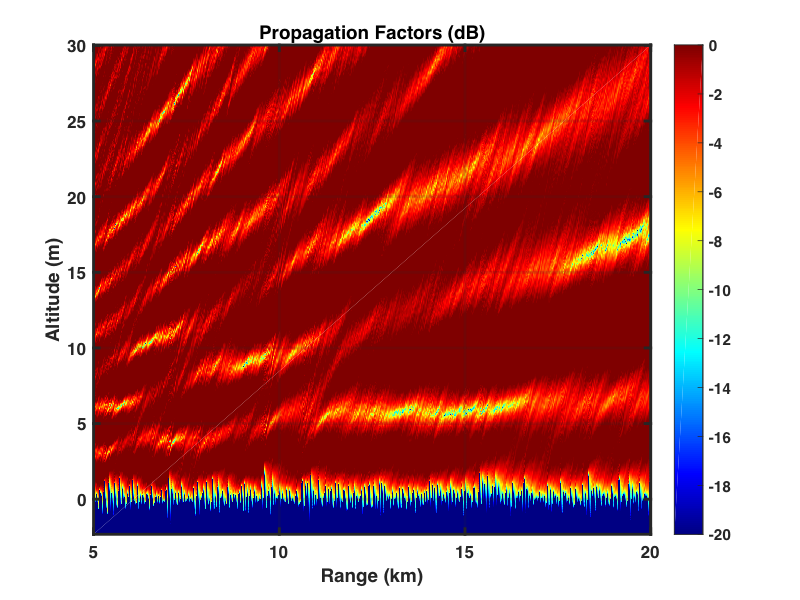
\includegraphics[width=4in]{../media/statistics/pf_1.png}
  \end{center}
  \renewcommand{\baselinestretch}{1} \small\normalsize
  \begin{quote}
    \caption[Example Propagation Factor Realization]{Example Propagation Factor Realization\label{stat_fig:1a}}
  \end{quote}
\end{figure}
\renewcommand{\baselinestretch}{2} \small\normalsize

\begin{figure}[H]
  \begin{center}
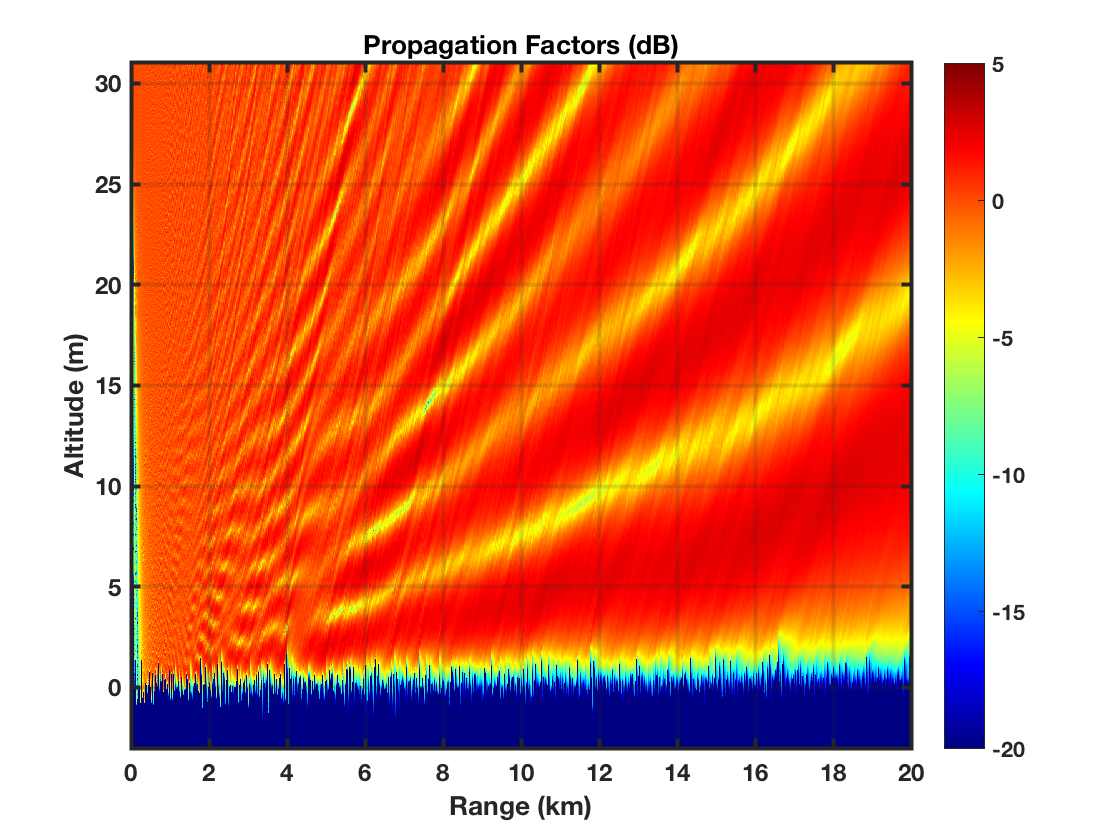
\includegraphics[width=4in]{../media/statistics/pf_2.png}
  \end{center}
  \renewcommand{\baselinestretch}{1} \small\normalsize
  \begin{quote}
    \caption[Example Propagation Factor Realization]{Example Propagation Factor Realization\label{stat_fig:1b}}
  \end{quote}
\end{figure}
\renewcommand{\baselinestretch}{2} \small\normalsize

\section{General Monte Carlo Results}
The mean and standard deviation with a 5 m/s wind speed and a $0^\circ$ wind direction are shown in Figure \ref{stat_fig:1zz} for standard atmosphere, and in Figure \ref{stat_fig:1zzz} for a 20 m duct.

\begin{figure}[H]
  \begin{center}
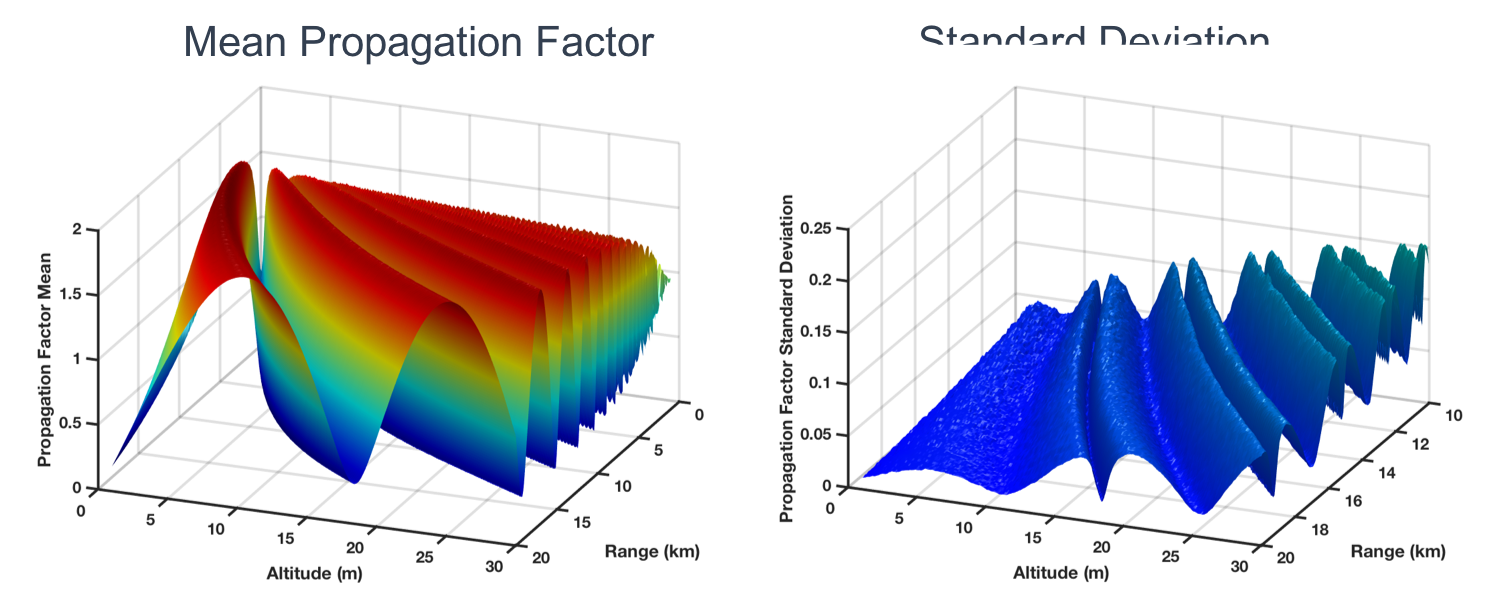
\includegraphics[width=4in]{../media/multistatic/std_atmos_results.png}
  \end{center}
  \renewcommand{\baselinestretch}{1} \small\normalsize
  \begin{quote}
    \caption[Standard Atmosphere Statistics at 5 m/s and $0^{\circ}$ Wind]{Standard Atmosphere Statistics at 5 m/s and $0^{\circ}$ Wind\label{stat_fig:1zz}}
  \end{quote}
\end{figure}
\renewcommand{\baselinestretch}{2} \small\normalsize

\begin{figure}[H]
  \begin{center}
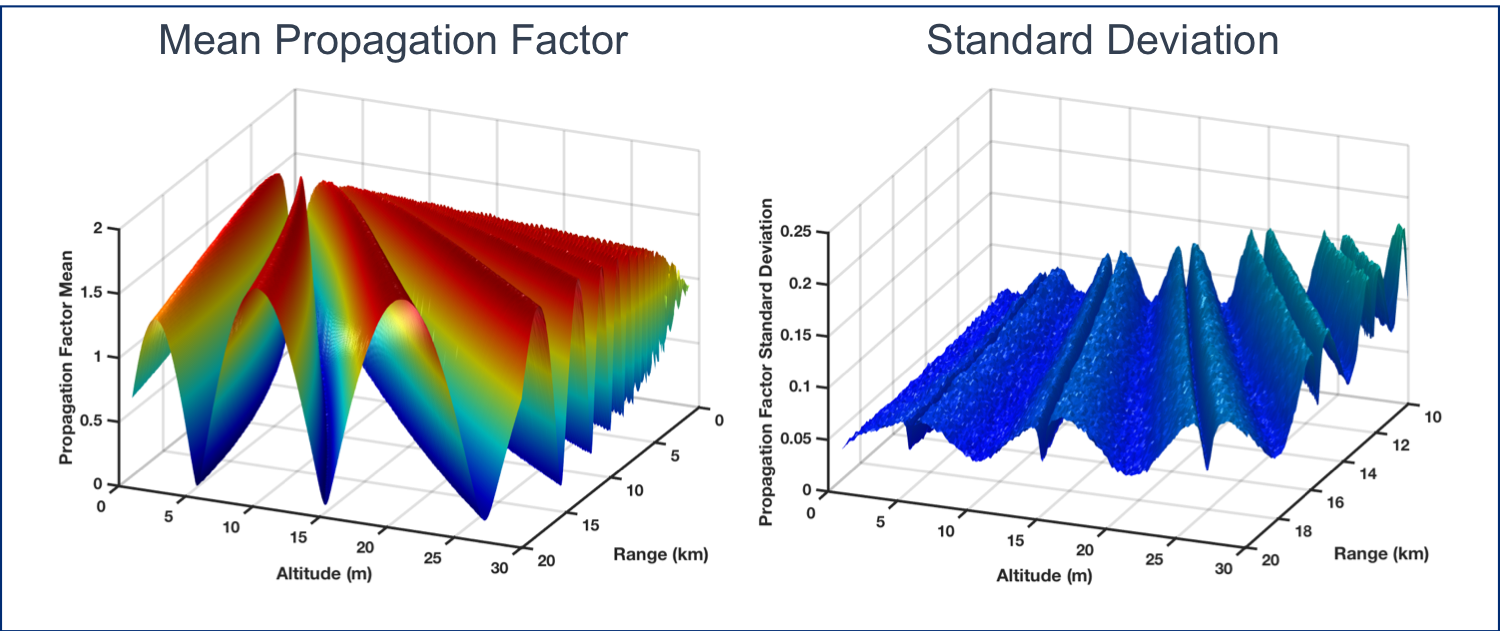
\includegraphics[width=4in]{../media/multistatic/duct_results.png}
  \end{center}
  \renewcommand{\baselinestretch}{1} \small\normalsize
  \begin{quote}
    \caption[20 m Duct Statistics at 5 m/s and $0^{\circ}$ Wind]{20 m Duct Statistics at 5 m/s and $0^{\circ}$ Wind\label{stat_fig:1zzz}}
  \end{quote}
\end{figure}
\renewcommand{\baselinestretch}{2} \small\normalsize

\begin{figure}[H]
  \begin{center}
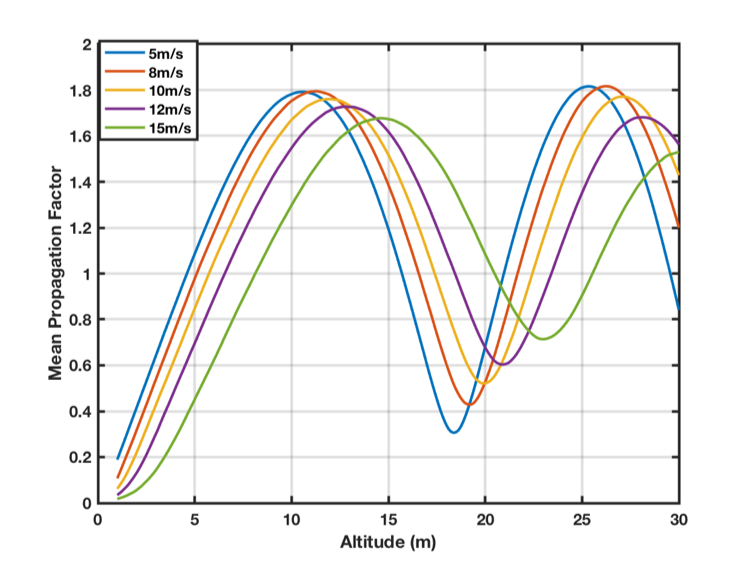
\includegraphics[width=4in]{../media/statistics/phase_shift_wind_speed.png}
  \end{center}
  \renewcommand{\baselinestretch}{1} \small\normalsize
  \begin{quote}
    \caption[Phase Shift at Constant Range due to Wind Speed]{Phase Shift at Constant Range due to Wind Speed\label{stat_fig:2zz}}
  \end{quote}
\end{figure}
\renewcommand{\baselinestretch}{2} \small\normalsize

\begin{figure}[H]
  \begin{center}
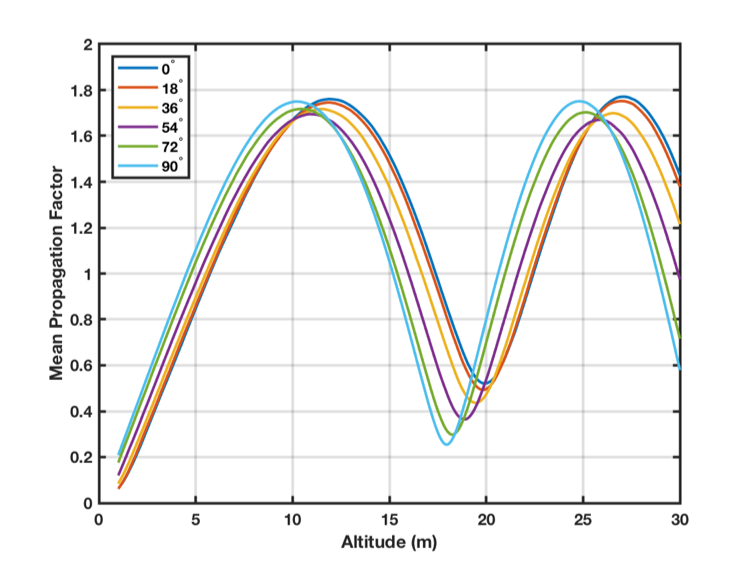
\includegraphics[width=4in]{../media/statistics/phase_shift_wind_direction.png}
  \end{center}
  \renewcommand{\baselinestretch}{1} \small\normalsize
  \begin{quote}
    \caption[Phase Shift at Constant Range due to Wind Direction]{Phase Shift at Constant Range due to Wind Direction\label{stat_fig:2zzz}}
  \end{quote}
\end{figure}
\renewcommand{\baselinestretch}{2} \small\normalsize

\section{PDF Fitting Results}
As shown in \cite{yeh_first_principles} and \cite{yeh_fading}, we expect the statistics to follow a Rician distribution
\begin{equation}
P = \frac{x}{\sigma^2}\exp\left[\frac{-(x^2 + \nu^2}{2\sigma^2} \right]I_0\left(\frac{x\nu}{\sigma} \right)
\label{stat_eq:5}
\end{equation}
\renewcommand{\baselinestretch}{2} \small\normalsize

This distribution has been previously shown to be applicable to modeling the amplitude statistics of multipath fading in communication systems with a strong direct line of sight path.

\subsection{Example Fitting Metrics}
\begin{figure}[H]
  \begin{center}
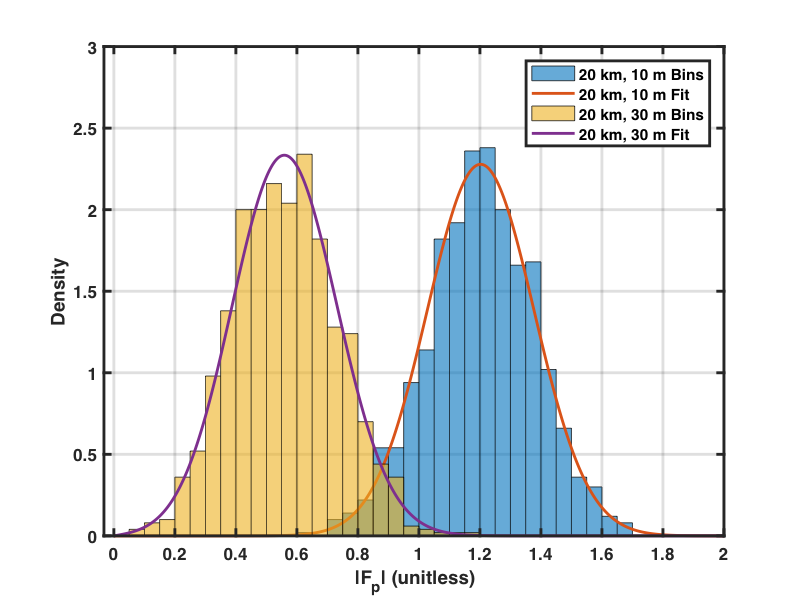
\includegraphics[width=4in]{../media/statistics/constant_range_fit.png}
  \end{center}
  \renewcommand{\baselinestretch}{1} \small\normalsize
  \begin{quote}
    \caption[PDF Fitting at Constant Range]{PDF Fitting at Constant Range\label{stat_fig:4}}
  \end{quote}
\end{figure}
\renewcommand{\baselinestretch}{2} \small\normalsize

\begin{figure}[H]
  \begin{center}
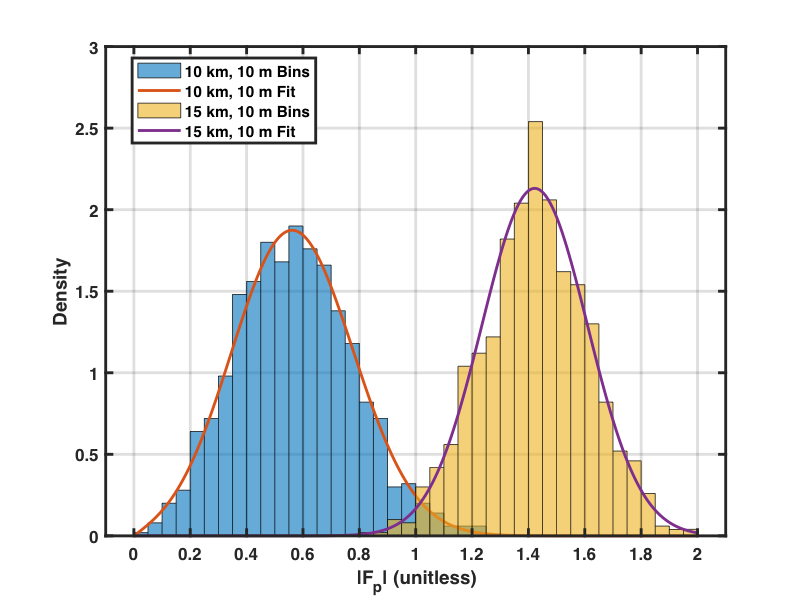
\includegraphics[width=4in]{../media/statistics/constant_altitude_fit.png}
  \end{center}
  \renewcommand{\baselinestretch}{1} \small\normalsize
  \begin{quote}
    \caption[PDF Fitting at Constant Altitude]{PDF Fitting at Constant Altitude\label{stat_fig:5}}
  \end{quote}
\end{figure}
\renewcommand{\baselinestretch}{2} \small\normalsize